%%%%%%%%%%%%%%%%%%%%%%%%%%%%%%%%%%%%%%%%%%%%%%%%%%
%
%  New template code for TAMU Theses and Dissertations starting Fall 2012.  
%  For more info about this template or the 
%  TAMU LaTeX User's Group, see http://www.howdy.me/.
%
%  Author: Wendy Lynn Turner 
%	 Version 1.0 
%  Last updated 8/5/2012
%
%%%%%%%%%%%%%%%%%%%%%%%%%%%%%%%%%%%%%%%%%%%%%%%%%%%
%%%%%%%%%%%%%%%%%%%%%%%%%%%%%%%%%%%%%%%%%%%%%%%%%%%%%%%%%%%%%%%%%%%%%%
%%                           SECTION IV
%%%%%%%%%%%%%%%%%%%%%%%%%%%%%%%%%%%%%%%%%%%%%%%%%%%%%%%%%%%%%%%%%%%%%

\chapter{\uppercase{Design}}

The main goal of Seismic Data Analytics SDK is to implement a distributed software development toolkit to enable scalable storage, computation and analytics for big seismic volume datasets. This chapter introduces the software architecture design and main functionalities of this toolkit.

\section{Software Architecture Design}

Seismic Data Analytics SDK is built upon Apache Hadoop and Spark. Figure \ref{sdk_swstack} shows the software stack of a workable seismic data analytics platform. In this diagram, the gray part is the OS layer, the elements with green color form the infrastructure layer, and on top of that the SDK layer consists of the components with blue color. At the bottom of the infrastructure layer, there is Hadoop Distributed File System (HDFS) that stores the big seismic data files by utilizing the large number of local disks. The Cassandra as a NoSQL database is also used to store seismic data, intermediate results and meta data. YARN and Mesos are used for resources management. Apache Spark is the data distribution and parallel execution engine based on the innovative idea of Resilient Distributed DataSets (RDD) concept. MLLib is included in the Spark as the machine learning package to enable machine learning based data analytics algorithms. OpenCV is the widely used image processing package that is used to provide image processing capability. Breeze is the numerical processing package including linear algebra, signal processing, statistics, and other numerical computation and optimizations developed in Scala. We have implemented the seismic data RDD on top of Spark as the base distributed seismic data collection to enable parallel operations and geophysical computations. Geophysicists and data scientists can use its interface to develop their own applications and leverage the capability of Apache Spark, as well as image processing, numerical computation, and deep learning packages.

\begin{figure}[h]
\centering
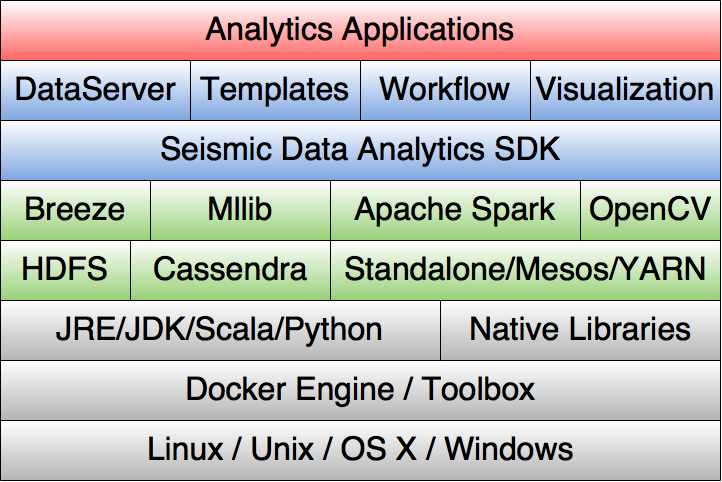
\includegraphics[scale=0.4]{figures/sdk_swstack.png}
\caption{Software Stack of Seismic Data Analytics Platform}
\label{sdk_swstack}
\end{figure}

Figure \ref{sdk_framework} simplifies the development efforts for scalable and distributed computation and analytics of seismic datasets. This toolkit is built on top of Apache Hadoop and Spark. The Hadoop provides a distributed file system(HDFS) and resource management system (YARN and Mesos), while Spark provides a high-level distributed data representation which is implemented by using Resilient Data Sets (RDD),  and a data-parallelism execution engine. Seismic Data Analytics SDK provides variety of configurable data distribution fashions for seismic volume data, as well as a user-defined parallel execution interface to simplify the parallel programming efforts. Furthermore, based on the base functionalities of SDK, we developed two useful utilities, parallel templates and data server, to facilitate SDK for users to easily deploy their applications. Since Hadoop and Spark are able to monitor and manage faults, resources and tasks schedule, the toolkit inherits from them also provides hight fault tolerance and dynamic task scheduling for better reliability and task management.

\begin{figure}[h]
\centering
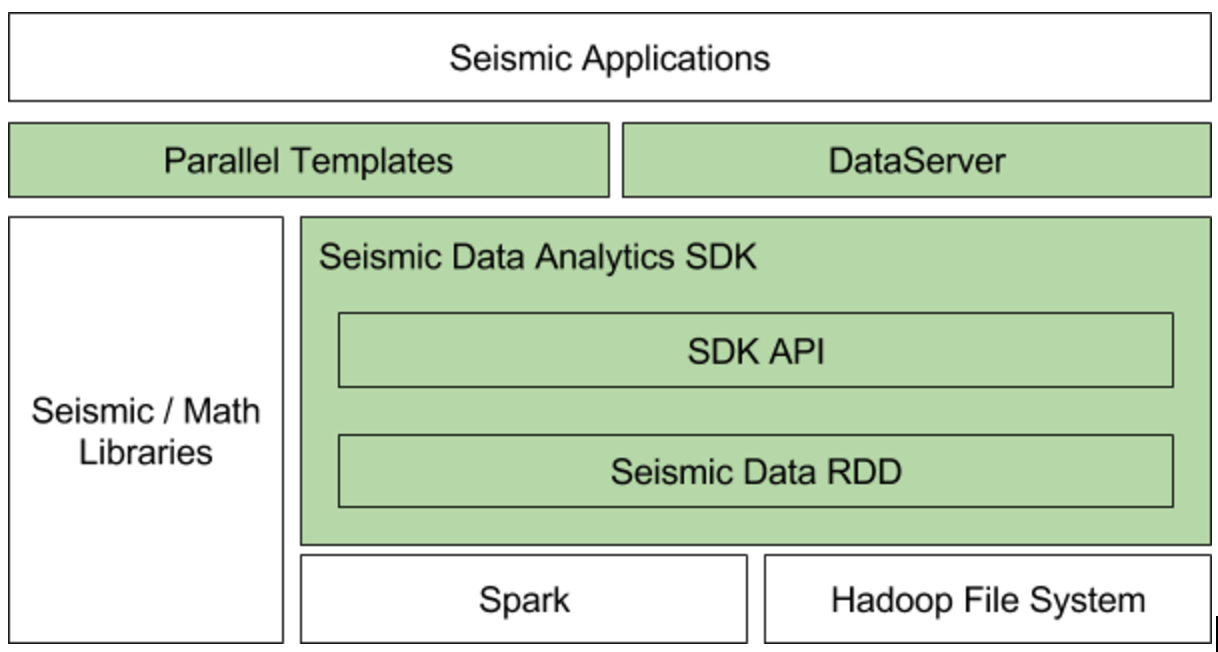
\includegraphics[scale=0.6]{figures/sdk_framework.png}
\caption{Framework of Seismic Data Analytics SDK}
\label{sdk_framework}
\end{figure}


\section{Interfaces and Functionalities}

Figure \ref{sdk_interface} shows the main functionalities of Seismic Data Analytics SDK, including data loading/saving, configurable distribution, data accessing, 3D transpose and user-defined function mapping. It provides a class \emph{SeismicVolume}, which integrates all the APIs of SDK, as the only public interface for users. Developers are able to create \emph{SeismicVolume} instances for specified seismic dataset, access data by configurable grain, perform 3D transposing, as well as apply user function to the distributed data instance, then finally save the application result to HDFS through the \emph{save()} function. The valid input data format include 3D binary data and SEG-Y file \cite{SEGDREV21} which is one of the most widely used standard format for the seismic data in petroleum industry.

\begin{figure}[h]
\centering
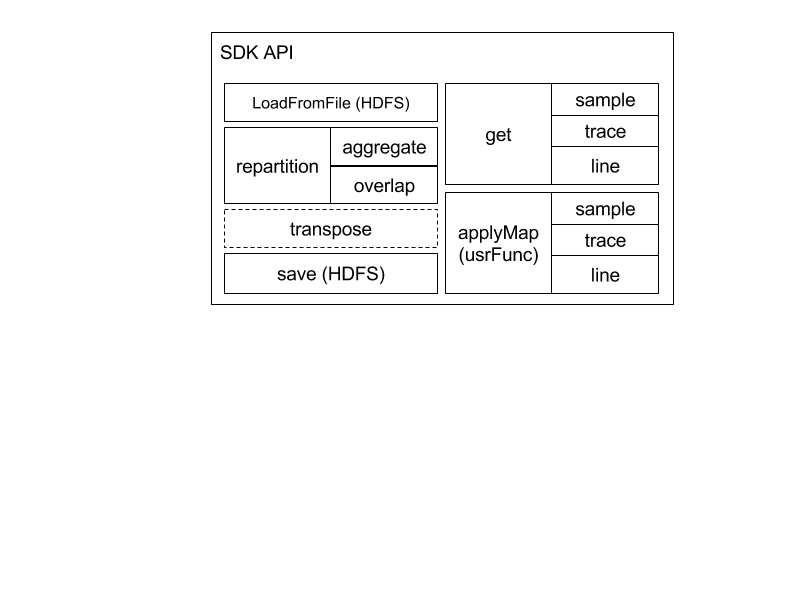
\includegraphics[scale=0.6]{figures/sdk_interface.png}
\caption{The Base APIs of Seismic Data Analytics SDK}
\label{sdk_interface}
\end{figure}

\section{Programming Language}

The host programming language of Seismic Analytics SDK is Scala, and the applications can be developed in Java. Scala (The acronym for Scalable Language), an object-oriented and functional language, provides great scalability in developing safe and high efficient multi-threaded applications \cite{ScalaOrg}. The most important reason of adopting Scala as the host language of SDK is it is also the native language of Apache Spark. It means Scala is the most efficient choices of this project. Moreover, Scala runs on JVM, which determines it can be freely integrated with Java. Also, the third party Java libraries and tools can be easily integrated with SDK. Since Scala compiler contains a subset of a Java compiler, Seismic Analytics SDK allows users who are not familiar with Scala or have strong Java preference can develop their applications in Java. This feature makes it possible for developers in industry to port the legacy Java applications to Seismic Analytics SDK without putting extra efforts on learning a new programming language.
